% --------------------------------------------------------------
% gabarito feito + 12 exercícios convertidos para múltipla escolha
% --------------------------------------------------------------
 
\documentclass[12pt]{article}\documentclass[brazilian,12pt,a4paper,final]{article}
\usepackage[brazil]{babel}
\usepackage[utf8]{inputenc}
\usepackage{graphicx}
\usepackage{color}
\usepackage{setspace}
\usepackage{ulem} 
\usepackage[margin=1in]{geometry} 
\usepackage{amsmath,amsthm,amssymb}
\usepackage{enumitem}
\newcommand{\N}{\mathbb{N}}
\newcommand{\Z}{\mathbb{Z}}
 
\newenvironment{theorem}[2][Theorem]{\begin{trivlist}
\item[\hskip \labelsep {\bfseries #1}\hskip \labelsep {\bfseries #2.}]}{\end{trivlist}}
\newenvironment{lemma}[2][Lemma]{\begin{trivlist}
\item[\hskip \labelsep {\bfseries #1}\hskip \labelsep {\bfseries #2.}]}{\end{trivlist}}
\newenvironment{exercise}[2][Exercise]{\begin{trivlist}
\item[\hskip \labelsep {\bfseries #1}\hskip \labelsep {\bfseries #2.}]}{\end{trivlist}}
\newenvironment{reflection}[2][Reflection]{\begin{trivlist}
\item[\hskip \labelsep {\bfseries #1}\hskip \labelsep {\bfseries #2.}]}{\end{trivlist}}
\newenvironment{proposition}[2][Proposition]{\begin{trivlist}
\item[\hskip \labelsep {\bfseries #1}\hskip \labelsep {\bfseries #2.}]}{\end{trivlist}}
\newenvironment{corollary}[2][Corollary]{\begin{trivlist}
\item[\hskip \labelsep {\bfseries #1}\hskip \labelsep {\bfseries #2.}]}{\end{trivlist}}
 
\begin{document}
 
 
\title{Exercícios}%replace X with the appropriate number
\author{\\ %replace with your name
MAT02219 - Probabilidade e estatística} %if necessary, replace with your course title
 
\maketitle
 \begin{enumerate} 
 %começo do capítulo 3

\section{CAPÍTULO 3}

 \item (área 1 - graficos) Cerca de 1\% das famílias na figura tem renda entre \$0 e \$1000.
 
 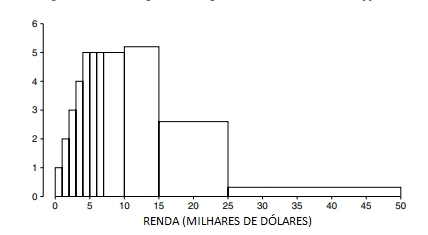
\includegraphics{Figuras/3A1.png}
 
 Estime a porcentagem que tem renda
 \begin{enumerate}[label=\Roman*]
     \item Entre \$1000 e \$2000
     \item Entre \$2000 e \$3000
     \item Entre \$3000 e \$4000
     \item Entre \$4000 e \$5000
     \item Entre \$4000 e \$7000
     \item Entre \$7000 e \$10000
\end{enumerate}
As porcentagens são, respectivamente:
\begin{enumerate}[label=(\alph*)]
\item 4\%, 2\%, 6\%, 5\%, 12\%, 18\%
\item 2\%, 3\%, 4\%, 5\%, 15\%, 15\%
\item 5\%, 2\%, 6\%, 4\%, 14\%, 20\%
\item 2\%, 3\%, 7\%, 8\%, 12\%, 10\%
\item 6\%, 1\%, 8\%, 3\%, 15\%, 15\%

\end{enumerate}
\textbf{Gabarito:(b) (I) 2\% (II) 3\% (III) 4\% (IV) 5\% (V) 15\% (VI) 15\%

}

\item (área 1 - gráficos) Na figura do exercício anterior, %haviam mais famílias ganhando entre \$10000 e \$11000 ou entre \$15000 e \$16000? Ou os números eram quase iguais? Dê o seu melhor palpite.

\begin{enumerate}[label=(\alph*)]
\item Haviam mais famílias ganhando entre \$10.000 e \$11.000 do que entre \$15.000 e \$16.000
\item Haviam mais famílias ganhando entre \$15.000 e \$16.000 do que entre \$10.000 e \$11.000
\item Havia o mesmo número de famílias ganhando entre \$10.000 e \$11.000 e entre \$15.000 e \$16.000, e esse número é maior do que o número de famílias ganhando entre \$5.000 e \$6.000.
\item Havia o mesmo número de famílias ganhando entre \$10.000 e \$11.000 e entre \$15.000 e \$16.000, mas esse número é menor do que o número de famílias ganhando entre \$5.000 e \$6.000.
\item Nenhuma das alternativas anteriores

\end{enumerate}

  \textbf{Resposta:(a) Mais entre \$10.000 e \$11.000}
 
\newpage
\item (área 1 - gráficos) O histograma abaixo mostra a distribuição das notas finais em uma determinada turma.

 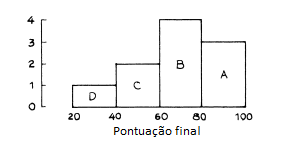
\includegraphics{Figuras/3A3.png}
 
\begin{enumerate}[label=(\Roman*)]
\item Qual bloco representa as pessoas que pontuaram entre 60 e 80?
\item Dez por cento pontuaram entre 20 e 40. Qual a porcentagem dos que tiraram entre 40 e 60?
\item Qual porcentagem pontuou mais de 60?
\end{enumerate}
As respostas para essas perguntas são, respectivamente,
\begin{enumerate}[label=(\alph*)]
\item B, 20\%, 50\%
\item A, 15\%, 60\%
\item B, 25\%, 60\%
\item B, 20\%, 70\%
\item C, 10\%, 70\%

\end{enumerate}
\textbf{Resposta: (d) (I) B (II) 20\% (III) 70\%}

\item (área 1 - gráficos) Abaixo estão esboços de histogramas para resultados de testes em três diferentes turmas. As pontuações variam de 0 a 100 e a nota necessária para aprovação é 50.

 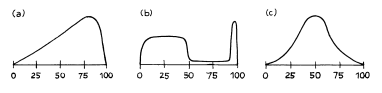
\includegraphics{Figuras/3A4.png}
 
Respectivamente, em cada turma, a porcentagem dos que passaram foi de:

\begin{enumerate}[label=(\alph*)]
\item Bem abaixo de 50\%, bem acima de 50\%, aproximadamente 50\%.
\item Bem acima de 50\%, bem acima de 50\%, bem abaixo de 50\%. 
\item Bem acima de 50\%, bem abaixo de 50\%, aproximadamente 50\%. 
\item Bem acima de 50\%, bem abaixo de 50\%, bem acima de 50\%. 
\item Nenhuma das alternativas anteriores.
\end{enumerate}

\textbf{Resposta:Alternativa (c) - Turmas: (a) Bem acima de 50\%. (b) Bem abaixo de 50\%. (c) Aproximadamente 50\%.}

\item (área 1 - gráficos) No exercício 4, pelo menos uma das turmas tinha dois grupos bem distintos de alunos, com um grupo
indo mal no teste, e o outro grupo indo muito bem. As turmas que tem essa característica são:

\begin{enumerate}[label=(\alph*)]
\item Turma (a)
\item Turma (b)
\item Turma (c)
\item Turmas (a) e (b)
\item Turmas (b) e (c)
\end{enumerate}

\textbf{Resposta:(b) turma (b)}

\item (área 1 - gráficos)
Na turma (b) do exercício 4, havia mais pessoas>

\begin{enumerate}[label=(\alph*)]
\item Com pontuação na faixa de 90 a 100 do que na de 40 a 50.
\item Com pontuação na faixa de 40 a 50 do que na de 90 a 100.
\item O número de pessoas com pontuação nas faixas de 40 a 50 e 90 a 100 é aproximadamente o mesmo, e é maior do que o número de pessoas com pontuação na faixa de 0 a 10.
\item O número de pessoas com pontuação nas faixas de 40 a 50 e 90 a 100 é aproximadamente o mesmo, e é menor do que o número de pessoas com pontuação na faixa de 0 a 10.
\item Nenhuma das alternativas anteriores.

\end{enumerate}


\textbf{Resposta:(a) Havia mais na faixa de 90 a 100}

\item (área 1 - gráficos)
São coletados dados sobre salários por hora para três grupos de pessoas. Aqueles que estão
no grupo B ganham
cerca do dobro dos que estão no grupo A. Os do grupo C ganham
cerca de \$ 10 por hora a mais do que os do grupo A. Qual histograma pertence a qual
grupo? (Os histogramas não mostram salários acima de \$ 50 por hora.)

 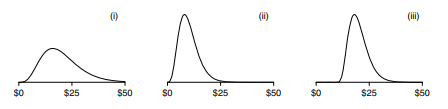
\includegraphics{Figuras/3A7.png}
 
 \begin{enumerate}[label=(\alph*)]
\item A (ii), B (iii), C (i)
\item A (i), B (ii), C (iii)
\item A (iii), B (i), C (ii)
\item A (iii), B (ii), C (i)
\item A (ii), B (i), C (iii)
 \end{enumerate}
 
\textbf{Resposta:(e) A (ii), B (i), C (iii)}

\item (área 1 - gráficos - ) A figura abaixo compara os histogramas para a renda familiar nos EUA em 1973
e em 2004. 

 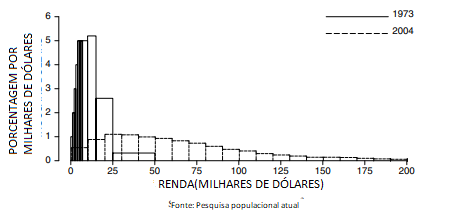
\includegraphics{Figuras/3A8.png}
 
Parece que a renda familiar aumentou 4 vezes em 30 anos. Ou será que não? Discuta brevemente.

\begin{enumerate}[label=(\alph*)]
    \item A renda aumentou 4 vezes em 30 anos, e não há nenhum outro fator a ser considerado.
    \item A renda média permaneceu a mesma, a diferença aparece somente na amplitude da distribuição.
    \item A renda aumentou 4 vezes em 30 anos, portanto há algo errado com os dados.
    \item A renda aumentou 4 vezes em 30 anos, porém a figura não ajusta a inflação, então não é uma boa comparação.
    \item Nenhuma das alternativas anteriores.
    
\end{enumerate}

\textbf{Resposta:(d) A figura não ajusta a inflação, então não é uma boa comparação.}


\iffalse
%%%%(Comentário:
%%%%questões difíceis de serem transformadas em múltipla escolha.)

\item (área 1 - tabelas) A tabela abaixo mostra a distribuição do nível educacional para pessoas com 25 anos ou mais
nos EUA em 1960, 1970 e 1991. 

 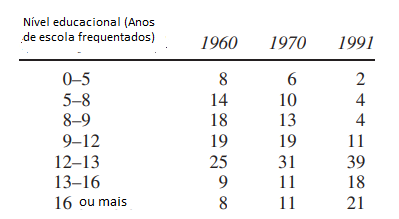
\includegraphics{Figuras/3B1.png}
 
("Nível educacional" significa o número de anos de escolaridade.) Os intervalos das aulas incluem o ponto final esquerdo,
mas não o direito; por exemplo, a partir da segunda linha da tabela, em 1960, cerca de 
14\% das pessoas completaram 5 a 8 anos de escolaridade, com 8 não incluídas; em 1991,
cerca de 4\% das pessoas estavam nessa categoria. Desenhe um histograma para os dados de 1991.
Você pode interpretar “16 ou mais” como 16 a 17 anos de escolaridade; poucas pessoas
completaram mais de 16 anos de escolaridade, especialmente em 1960 e 1970. Por que
seu histograma tem picos aos 8, 12 e 16 anos de escolaridade?


\item Redesenhe o histograma do exercício anterior para os dados de 1991, combinando os dois primeiros intervalos de classe em
um (0 a 8 anos, com 6\% da população). Isso muda muito o histograma?

\item 
Desenhe o histograma para os dados de 1970 e compare com o histograma de 1991. O que
aconteceu com o nível educacional da população entre 1970 e 1991 - ele subiu, desceu ou permaneceu o mesmo?
%%%%fim do comentário
\fi 
%o próximo exercício pode virar múltipla escolha usando a tabela 3B1.png

\item 
(área 1 - tabela - comportamento de uma varíavel no tempo) Quanto ao nível educacional, é possível afirmar que:
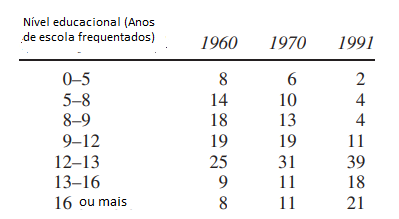
\includegraphics{Figuras/3B1.png}
\begin{enumerate}[label=(\alph*)]
\item O nível educacional subiu de 1960 a 1970. 
\item O nível educacional decresceu de 1960 a 1970.
\item O nível educacional permaneceu o mesmo de 1960 a 1970 e aumentou de 1970 a 1991.
\item O nível educacional permaneceu o mesmo de 1960 a 1970 e decresceu de 1970 a 1991.
\item Nenhuma das alternativas anteriores.
\end{enumerate}
\textbf{Resposta:(a) O nível educacional subiu. Por exemplo, mais pessoas terminaram o ensino médio e
ingressaram na faculdade em 1991 do que em 1970.
}

\item (área 1 - gráficos - histograma) Um histograma de salários mensais para funcionários de meio período é mostrado abaixo (densidades
estão marcados entre parênteses).

 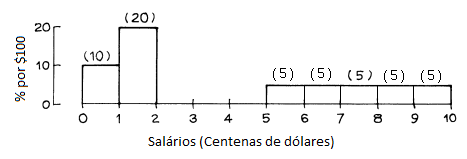
\includegraphics{Figuras/3C1.png}
 
Ninguém ganhava mais de US\$ 1.000 por mês. Os blocos
no intervalo da classe de US \$ 200 a US \$ 500 estão ausentes. Quais devem ser as suas alturas?

\begin{enumerate}[label=(\alph*)]
\item 25\% por \$100.
\item 20\% por \$100.
\item 15\% por \$100.
\item 10\% por \$100.
\item 5\% por \$100.
\end{enumerate}

\textbf{Resposta:(c) 15\% por \$100.}

\item(área 1 - gráficos) Três pessoas plotam histogramas para os pesos das cobaias de um estudo, usando a escala de densidade.

 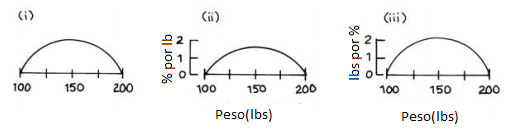
\includegraphics{Figuras/3C2.png}
 
 Estão certos:
 \begin{enumerate}[label=(\alph*)]
\item Apenas (i).
 \item Apenas (ii).
 \item Apenas (iii).
 \item Apenas (ii) e (iii).
 \item Todos estão certos.
 \end{enumerate}
 \textbf{Gabarito:Opção (c) (ii) é a resposta, pois (i) não tem unidade e (iii) tem a unidade errada para densidade.}
 
\item (área 1 - Unidades e porcentagens) Uma investigadora desenha um histograma para alguns dados de altura, usando o sistema métrico.
Ela está trabalhando em centímetros (cm). O eixo vertical mostra a densidade e a parte superior
do eixo vertical é de 10\% por cm. Agora ela quer converter para milímetros. Existem 10 milímetros em 1 centímetro. No eixo horizontal, ela precisa
alterar 175 cm para \_\_\_ mm e 200 cm para \_\_\_ mm. No eixo vertical,
ela precisa mudar 10\% por cm para \_\_\_ \% por mm e 5\% por
cm para \_\_\_ \% por mm.
Respectivamente, as respostas que preenchem os espaços em branco são:
\begin{enumerate}[label=(\alph*)]
\item 17500; 20000; 1; 0,5.
\item 1750; 2000; 0,1; 0,05.
\item 17500; 20000; 10; 5.
\item 17,5; 20; 1; 0,5.
\item 1750; 2000; 1; 0,5.
\end{enumerate}

\textbf{Respostas:(e) 1750; 2000; 1; 0,5.}


\item (área 1 - gráficos) Em um estudo do Serviço Público de Saúde, um histograma foi plotado mostrando o número
cigarros por dia fumados por cada cobaia (fumantes atuais), como mostrado
abaixo. A densidade é marcada entre parênteses. Os intervalos das classes incluem o ponto final à direita, não a esquerda.

 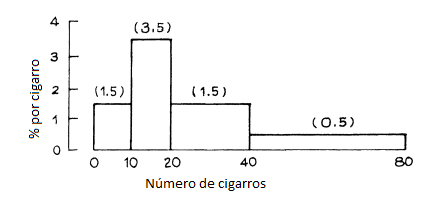
\includegraphics{Figuras/3C4.png}
\begin{enumerate}[label=(\Roman*)]
\item A porcentagem que fumava 10 cigarros ou menos por dia é de cerca de

%\hspace{4cm}1,5\%\hspace{0,8cm}15\%\hspace{0,8cm}30\%\hspace{0,8cm} 50\%

\item A porcentagem que fumava mais de um maço por dia, mas não mais que 2
pacotes, está em torno de


%\hspace{4cm}1,5\%\hspace{0,8cm} 15\% \hspace{0,8cm} 30\% \hspace{0,8cm} 50\%


(Existem 20 cigarros em um maço.)
\item A porcentagem que fumava mais de um maço por dia é de cerca de

%\hspace{4cm}1,5\%\hspace{0,8cm} 15\%\hspace{0,8cm} 30\%\hspace{0,8cm} 50\%
\item A porcentagem que fumava mais de 3 maços por dia é de cerca de

%\hspace{4cm} 0,25 de 1\% \hspace{0,8cm} 0,5 de 1\% \hspace{0,8cm} 10\%
\item A porcentagem que fumava 15 cigarros por dia é de cerca de

%\hspace{2,5cm}0,35 de 1\% \hspace{0,8cm} 0,5 de 1\% \hspace{0,8cm} 1,5\% \hspace{0,8cm} 3,5\% \hspace{0,8cm} 10\%
\end{enumerate}
As respostas que completam cada frase são:
\begin{enumerate}[label=(\alph*)]
\item (I) 1,5\% (II) 15\% (III) 30\% (IV) 0,5 de 1\% (V) 10\%
\item (I) 15\% (II) 50\% (III) 30\% (IV) 10\% (V) 1,5\%
\item (I) 50\% (II) 15\% (III) 1,5\% (IV) 0,25 de 1\% (V) 3,5\%
\item (I) 30\% (II) 30\% (III) 50\% (IV) 10\% (V) 3,5\%
\item (I) 15\% (II) 30\% (III) 30\% (IV) 10\% (V) 1,5\%

\end{enumerate}

\textbf{Resposta:(d) (I) 1.5\% por cigarro × 10 cigarros = 15\%.
(II) 30\% (III) 30\% + 20\% = 50\% (IV) 10\% (V) 3.5\%}

\item (área 1 - classificação de variáveis) Classifique cada uma das seguintes variáveis como qualitativa ou quantitativa; se quantitativa, especifique se é discreta ou contínua.
\begin{enumerate}[label=(\Roman*)]
\item ocupação \item região de residência \item peso
\item altura \item número de automóveis próprios
\end{enumerate}

As classificações para cada variável são, respectivamente,
\begin{enumerate}[label=(\alph*)]
\item Qualitativa; qualitativa; quantitativa contínua; quantitativa discreta; quantitativa contínua.
\item Quantitativa contínua; qualitativa; quantitativa discreta; qualitativa; quantitativa discreta.
\item Qualitativa. quantitativa discreta; qualitativa; quantitativa discreta.
\item Quantitativa discreta; quantitativa contínua; qualitativa; qualitativa; quantitativa contínua.
\item Qualitativa; qualitativa; quantitativa contínua; quantitativa contínua; quantitativa discreta.
\end{enumerate}
\textbf{Respostas:(e) (I) qualitativa
(II) qualitativa
(III) quantitativa, contínua
(IV) quantitativa, contínua
(V) quantitativa, discreta}

\item (área 1 - tabelas) Numa pesquisa populacional, as mulheres foram questionadas quanto ao número de filhos que possuíam. Os resultados são mostrados abaixo para mulheres de 25 a 39 anos, por nível educacional.

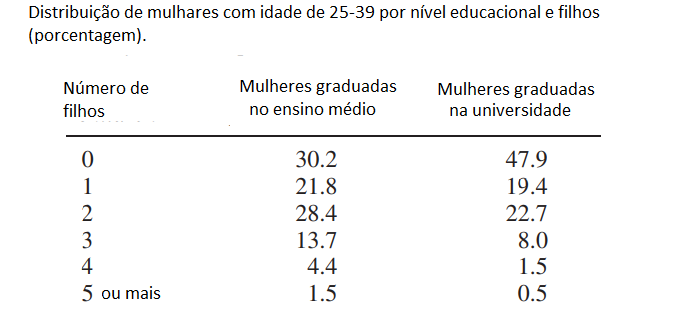
\includegraphics{Figuras/3D2.png}

 O número de filhos é discreto ou contínuo? O que pode ser concluido a partir dos dados? Desenhe um histograma, se achar necessário.
%\item Desenhe histogramas para esses dados. (Você pode usar "5 ou mais" como 5 - muito poucas
%mulheres tiveram mais de 5 filhos.)
% b não viável para múltipla escolha
\begin{enumerate}[label=(\alph*)]
\item Número de filhos é uma variável contínua. Mulheres com maior nível educacional tem menos filhos.
\item Número de filhos é uma variável discreta. Mulheres com menor nível educacional tem menos filhos.
\item Número de filhos é uma variável discreta. Mulheres com maior nível educacional tem menos filhos.
\item Número de filhos é uma variável contínua. Mulheres com menor nível educacional tem menos filhos.
\item Número de filhos é uma variável discreta. Não há diferença perceptível entre o número de filhos para os diferentes níveis educacionais.

\end{enumerate}


\textbf{Resposta:(c) Número de filhos é uma variável discreta. Mulheres com maior nível educacional tem menos filhos.}


\end{enumerate}
\end{document}